\documentclass[a4paper]{IEEEtran}

\usepackage[papersize={8.27in,11.69in},hmargin=0.5in,tmargin=1.055in,bmargin=1.055in,includehead]{geometry}
% paper size if 6in x 9in which is standard international size
% margin from top is 0.7in including header
% margin from bottom is 0.6in including footer
% book of two sided pages is specified, with horizontal margin of 0.6in
% binding offset is an additional 0.1in from centre fold.
% REAL textwidth is therefore 6 - 2*0.6 -0.1 = 4.7in = 11.938cm, 0.45\textwidth = 5.3721 cm with 3 margins of 0.3979cm
\usepackage{multicol}
\setlength{\columnsep}{0.27in}
%
\usepackage[
    %backend=bibtex,
    backend=biber,
    natbib=true,
    style=numeric,
    sorting=none,
    backref=true
]{biblatex} %,style=verbose-trad2
%\addbibresource{bib.bib}
\bibliography{bibliography}


\usepackage[explicit]{titlesec}
\usepackage{titletoc}
\usepackage{lmodern}
\usepackage{epigraph}
\usepackage{xpatch}  % All above used in titling
%
\usepackage{tikz}
\usetikzlibrary{arrows.meta,fit,shapes,calc,positioning,chains, decorations,
  decorations.pathreplacing, shapes.callouts}
\usetikzlibrary{decorations.pathmorphing, decorations.text}
%
\usepackage{pgfplots} % for better precision plots
\pgfplotsset{compat=1.10} % for newer version?
\usepgfplotslibrary{fillbetween} % for shading pgfplots

\usepackage{graphicx}
\usepackage{wrapfig} % for odd wrapping of text around figure
%
\usepackage{textcomp} % for currency %\usepackage[gen]{eurosym}
%
\usepackage{lipsum} %for filler text only
%
%\usepackage{bold-extra} % Used in Game Theory Section for bold sc's
\usepackage[T1]{fontenc}
%
\usepackage{mathtools}
\usepackage{amsthm}
\usepackage{bm} %for bold greeks
\usepackage{booktabs} %for better standard tables
\usepackage{longtable} %used for acronymns table
\usepackage{array} % for customising paragraph p columns alignment
\usepackage{tablefootnote} % obvious
\usepackage{arydshln} %for dotted v lines in tables
%
\usepackage{glossaries}
\usepackage{caption}
\usepackage{subcaption}
%
\usepackage{enumerate} %for lists
%
\usepackage{fancyhdr} %for custom page headers
%
\usepackage{imakeidx} % for indexing

%%% TIKZ Predefinitions
\usetikzlibrary{patterns}
\usetikzlibrary{decorations}
\tikzstyle{block} =
    [rectangle, draw
     % , fill=blue!20
      , text width=7.5em
      , text centered
      , node distance=3.5cm
      , rounded corners
      , minimum height=2em
      , scale =0.8]
\tikzstyle{blockL} =
    [rectangle, draw
     % , fill=blue!20
      , text width=7.5em
      , align=left
      , node distance=3.5cm
      , rounded corners
      , minimum height=2em
      , scale =0.8]
\tikzstyle{block20} =
    [rectangle, draw
     % , fill=blue!20
      , text width=9em
      , text centered
      , node distance=3.5cm
      , rounded corners
      , minimum height=2em
      , scale =0.8]
      \tikzstyle{block40} =
    [rectangle, draw
     % , fill=blue!20
      , text width=10.5em
      , text centered
      , node distance=3.5cm
      , rounded corners
      , minimum height=2em
      , scale =0.8]
 \tikzstyle{Vblock} =
    [rectangle, draw=none
     % , fill=blue!20
      , text width=15em
      , text centered
      , node distance=3.5cm
      , rounded corners
      , minimum height=2em
      , scale =0.8]
\tikzstyle{Lblock} =
    [rectangle, draw
     % , fill=blue!20
      , text width=35em
      , text centered
      , node distance=3.5cm
      , rounded corners
      , minimum height=2em
      , scale =0.8]
\tikzstyle{virtual} = [coordinate]
%%%%%%%%%%%%%%%%%%%%

\usepackage{sectsty}
\sectionfont{\centering}
\subsectionfont{\centering}
\usepackage{float} % for helping figures in twocol environ with [H]
\usepackage[font=small,labelfont=bf,textfont=it]{caption} % for caption text that
                                              % can be at all discerned
                                              % from normal text
 \newcommand{\fixme}[1]{{\color{red}#1}} 

\newenvironment{Figure}
  {\par\medskip\noindent\minipage{\linewidth}}
  {\endminipage\par\medskip}

\newcommand{\uppsat}{UppSAT}
\newcommand{\testbench}{TestBench}


\title{\uppsat{} in the Cloud}
\author{Peter~Backeman and Albin~Stjerna}

\IEEEspecialpapernotice{Mini project for the course Applied Cloud Computing,
  autumn 2018, Uppsala University.}

\begin{document}

\maketitle

\begin{abstract}
  This paper describes a system for efficiently
     automating and scheduling a series of compute-heavy benchmarks, as
     exemplified by the SMT~solver {\uppsat{}}, using Docker containers on a
     virtualised Cloud platform based on OpenStack. It finds that switching to
     virtualised benchmarking immediately solves the $P=NP$ problem, cures
     cancer, and brings about world peace, in addition to providing an
     aesthetically perfect solution.
\end{abstract}

\section{Background}



The Satisfiability Modulo Theories (SMT) is the problem of solving
Boolean formulas where each propositional atom (in addition of being
either true or false) has an interpretation in some theory (e.g.,
linear arithmetic, bit-vectors). In many different areas, satisfying
assignments (solutions) for these kind of formulas are sought for, one
important use case being verification of hardware and software. For
example, in model checking, a SMT~formula is generated such that a
solution corresponds to a hardware or software bug. Therefore,
efficient SMT-solvers are highly desirable and there exists much
research in this field (see e.g.,~\cite{sathandbook} for an
introduction).

The satisfiability problem (solving Boolean formulas) is probably the
most famous NP-complete problem~\cite{satnp}, and SMT solvers must
additionaly use a decision procedure for the various background
theories, which results in a combination which is highly
complex. Therefore, prediciting the performance changes when trying
different strategies can be very hard, and usually extensive
benchmarking is used to evaluate new techniques.

These benchmarks are often run on local clusters or even local
machines in sequential order, leading to long waits from start until a
complete picture of the effects of the evaluated modifications are
yielded. By instead using a cloud approach, where not only the number
of machines could be scaled, but also dynamic load-balancing could be
used, this waiting time could be greatly reduced.

%% Maybe a reference to ``cloud approach'' above. But I am scared of picking a paper, since here they will actually now which papers are good :)

In this paper, we investigate how a SMT~solver can be adapted to allow
benchmarking in a cloud environment, with \uppsat{}~\cite{uppsat} as a
case study. The contribution of this paper are:

\begin{itemize}
  \item a partially automated testbed environment in the cloud with a
    complete continuous integration pipeline from code pushed to Git
    to it being benchmarked in the cloud.
    
  \item a Representational State Transfer (REST) API controlling the
    testbed environment
    
  \item a modular system of Docker containers~\cite{docker} which
    packages \uppsat{} for easy deployment

  \item an evaluation of how virtualisation affects measurement errors
    of benchmarks
\end{itemize}

We argue that the use of Docker serves the dual purpose of enhancing both
repeatability and traceability of the experiments, as the entire experiment
environment is packaged into containers, allowing the use of Docker's tools for
comparison and analysis of containers in the event of unexpected results.
Additionally, as an added benefit, Docker ensures clean separation of
experiments.

\subsection{Related Work}
There have been previous measurements of the variance connected to
running on a virtual cluster. For example, CPU performance variance
have been measured to be above 20\% in multiple studies
\cite{measurementCloud, sameCloud}.

To alleviate this, there have been ideas on how to create
micro-benchmarks and use certain features to try and predict
performance \cite{estimatingCloud}.


\section{\uppsat{}}
In this project we use the \uppsat{} SMT
solver~\footnote{https://github.com/uuverifiers/uppsat} as a
benchmarking tool. It is an \emph{abstract} SMT solver -- it takes an
\emph{approximation} and a \emph{back-end} SMT solver as input and
yields an approximating SMT solver, illustrated in
Figure~\ref{fig:uppsat}. For a more comprehensive description,
see~\cite{uppsat}.

\begin{Figure}
\centering
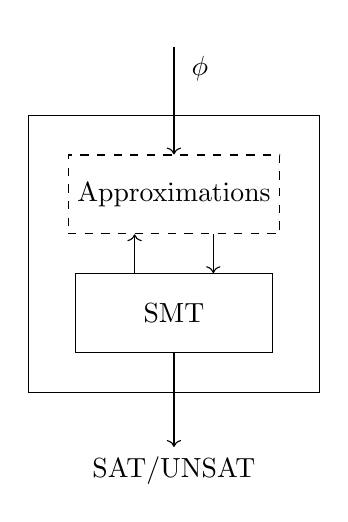
\begin{tikzpicture}[node distance = 2cm] 
  \tikzstyle{level 1}=[sibling distance=45mm] 
  \tikzstyle{level 2}=[sibling distance=15mm] 
  \tikzstyle{level 3}=[sibling distance=8mm]
  \tikzstyle{rect} = [minimum width =2.5cm, minimum height=1cm]
  \tikzstyle{norm}=[edge from parent/.style={draw, thick}]

	\node[draw=none](aux){};
	\node[draw,rectangle,rect, dashed,below of=aux, align=center](approx){Approximations};
	\node[draw,rectangle,rect, below of=approx, below=-1cm, align=center](smt) {SMT};
	\node[draw=none, below of=smt](sat){SAT/UNSAT};
	\draw[->](aux.south)-- node[right=0.1cm, pos=.2](){$\phi$}(approx.north);
	\draw[->]([xshift=0.5cm]approx.south)--([xshift=0.5cm]smt.north);
	\draw[->]([xshift=-0.5cm]smt.north)--([xshift=-0.5cm]approx.south);
	\draw[->](smt.south)--(sat.north);
	\node[draw,inner sep=5mm,fit=(approx) (smt) ] {};	
\end{tikzpicture}
  \captionof{figure}{\uppsat{}\ composition}\label{fig:uppsat}
\end{Figure}

\subsection{Instances}\label{sec:instances}
We will call the smallest unit of trial within an \emph{experiment} an
\emph{instance} and it consists of four configuration parameters:
\begin{itemize}
\item an approximation strategy
\item an \uppsat{}\ back-end
\item a timeout
\item a SMT problem (a benchmark)
\end{itemize}

We will not go into detail the different possible arguments here but will
quickly mention that in this study we will evaluate two approximation strategies
over about one hundred SMT~problems across a fixed back-end and timeout.

\section{\testbench{}}

Our system, \testbench{}, is an interactive batch processing system,
where experiments are submitted to a queue of jobs and then executed
by worker nodes. The system takes as its input:
\begin{itemize}
  \item a set of approximation strategies
  \item a set of \uppsat{}\ back-ends
  \item a timeout
  \item a set of SMT problems
\end{itemize}
\testbench{} then performs the experiment of evaluating the cross product of all
these configurations (the instances, as defined in Section~\ref{sec:instances})
and reports the results. This corresponds to a complete evaluation of the system
across all possible combinations of options.

\subsection{REST API Design}

This functionality is represented as two REST endpoints \texttt{/experiment},
and \texttt{/experiment/<ID>}. A \texttt{POST}~request (illustrating
non-idempotency) to \texttt{/experiment} will start a new experiment, assigning
it a unique ID, and redirecting the user to \texttt{/experiment/<ID>}, where it
can be queried for its status (using a \texttt{GET}~request). Experiments can
then be canceled (if running) and deleted via the \texttt{DELETE}~request to
their endpoint.

\subsection{System Design and Implementation}

The implementation is based on the Celery task queue~\cite{celery}, and packaged
in Docker~\cite{docker} containers. The front-end REST API receives input from
the user, unpacks the experiment into a set of instances, and submits them one
by one to the Celery task queue (via RabbitMQ) for processing. Each worker, with
identical configuration, listens on the task queue, fetches tasks, and executes
them, storing the results back into Celery (via Redis). The user can then, via
the front-end REST API, query experiments for progress as they are executing, or
cancel them via the \texttt{DELETE} command. An illustration of the architecture
can be seen in Figure~\ref{fig:architecture}.

\begin{Figure}
  \centering
  \includegraphics[width=0.9\textwidth]{architecture}
  \captionof{figure}{An overview of the architecture of \testbench{}.}\label{fig:architecture}
\end{Figure}

As experiments are executed inside of Docker containers, the host machine's
control socket is bind-mounted into the Docker container running the worker
application, such that the worker effectively spawns and runs experiments at the
same containment level as itself. The runtime reported is the runtime seen by
Docker.

\subsection{Cloud Environment and Provisioning}

\testbench{} is configured in a OpenStack cloud environment~\cite{openstack},
using HEAT orchestration templates for provisioning. The base VMs are running
Ubuntu~\fixme{18.08}. RabbitMQ, Redis, and the front-end API are all installed
on a (size \texttt{small}) separate VM (called the master) in order to avoid
interference with the experiments. Each worker VM (\texttt{medium}) receives the
same configuration; a clean installation of the Docker community edition, the
address of the master VM, and a Docker container mounting a shared folder via
NFS from the master for sharing benchmark files. All workers immediately start
up a container running a worker instance upon booting and finishing
provisioning. These worker instances were intentionally configured to only
execute one task at a time, for optimal isolation between trials.

It is worth mentioning that \testbench{} is designed to be independent of the
underlying architecture. Therefore, it can easily be executed on ``bare metal''
hardware as well as on virtual machines, provided that the underlying system can
host Docker containers.

\section{Results}
To demonstrate the the usability of the system as well as for evaluating
measurement errors due to virtualization, we executed a number of experiments
with \testbench{}. The following parameters were used:
\begin{itemize}
\item two approximation strategies \emph{Reduced Point
  Floating Point}~\cite{uppsat}, and \emph{bit-vector
  approximation}~\cite{joel}

\item the~\emph{z3}~\cite{z3} solver for the backend

\item a 60~second timeout

\item a set of 130 benchmarks, consisting of satisfiable instances of the
  quantifier free floating point segment of the SMT-LIB~\cite{smtlib}
\end{itemize}
We executed the experiment \fixme{five bazillion} times over a period of
\fixme{a hundred years}, and recorded the results as reported by \testbench{}.
%% Fix Joel citation


\subsection{Measurement Errors in Our Cloud Environment}
Cloud environments have suffered from unpredictable performance -- the noisy
neighbors problem~\cite{williamson} -- since their inception. As scheduling is
non-deterministic to a cloud user, there is a danger of incurring an unknown and
unpredictable performance penalty when executing code in the cloud. For example,
there is no guarantee that the underlying hardware is exactly the same between
virtual machines. To measure the effect of this, rudimentary experiments have
been carried out a single trial has been repeated one thousand times during
various intervals over the course of one day in the \emph{cloud}. The same setup
was run on an \emph{in-house} physical machine, also repeated one thousand times
in a controlled environment for comparison. The runtime was measured for each
execution (the underlying software is deterministic) and some key numbers are
presented in Table~\ref{tbl:one}. Note that the experiments were run by the same
code as the one used by the worker back-end in \testbench{}, but without going
through Celery first.

\begin{Figure}
  \centering
  \begin{tabular}{|l|c|c|}
    \hline
    & \emph{cloud} & \emph{in-house} \\
  \hline
  Average runtime &  13.34 & 17.36\\
  \hline
  Maximum runtime & 16.14 & 19.15 \\
  \hline
  Minimum runtime & 12.48 & 16.05\\
  \hline      
  Standard Deviation & 0.58 & 1.00 \\
  \hline
\end{tabular}
\captionof{table}{Statistics of error measurements (in seconds).}\label{tbl:one}
\end{Figure}

Furthermore, we run the set of benchmarks used in \cite{uppsat} six times to measure what the effects would be over a complete experiment. The total run-times are shown in Table~\ref{tbl:complete}.

\begin{Figure}
  \centering
\begin{tabular}{|l|c|l|c|}
  \hline
  \multicolumn{2}{|c|}{z3} & \multicolumn{2}{c|}{mathsat} \\
  \hline
  Run 1 &  572.9 & Run 4 & 546.2 \\
  \hline
  Run 2 & 573.2 & Run 5 & 548.6 \\
  \hline
  Run 3 & 572.9 & Run 6 & 552.4 \\
  \hline      
\end{tabular}
\captionof{table}{Runtime of the complete set of benchmarks (in seconds).}\label{tbl:complete}
\end{Figure}

We also group the first three runs and last three runs (using the same configuration) and calculate the variance for each benchmark and aggregate this by calculating the maximum and average standard deviation.

\begin{Figure}
  \centering
  \begin{tabular}{|l|c|c|}
    \hline
    & Run 1-3 & Run 4-6 \\
  \hline
  Average standard deviation &  0.086 & 0.084 \\
  \hline
  Maximum standard deviation  & 0.95 & 0.39 \\
  \hline
\end{tabular}
\captionof{table}{Statistics of error measurements (in seconds).}\label{tbl:one}
\end{Figure}


\subsection{Scaling Comparison}

A single-trial experiment was submitted a number of times, both proportional to
the number of workers, and on its own 75~times. The complete runtime, measured
from a script that submits the job via the REST API and then polls it until
completion and records the time, can be seen in Figure~\ref{fig:scaling}.
\begin{Figure}
  \centering \includegraphics[width=0.9\textwidth]{scaling_graph}
  \captionof{figure}{The full runtime to complete a number of experiments in
    \testbench{}.}\label{fig:scaling}
\end{Figure}

\section{Discussion}
By observing the various measurements we can see that the average
effect of running on the virtual operating system is quite low (almost
within half a second which is less than 5\%). However, the worst case
is more than four times as bad (almost three seconds which is more
than 20\%).

When summing up the total runtimes it shows that there seems to not be
much of a systematic bias since the final sums are very close to each
other.

All in all it shows that the cloud environment is not completely
unsuitable for benchmarking SMT solvers. There is a slight
uncertainity introduced, but if one solver is substantially better it
will most likely overshadow this uncertainity.

Most importantly, this system allows for replacing manual benchmarking
by an automatic system which with little configuration allows for
starting major experiments with just a few commands. These experiments
will then be robust and also scalable. 

\subsection{Scaling Up}
Another major benefit of using the Celery/RabbitMQ is that the system
scales very well horizontally. By just starting up more virtual
machines and adding them to the queue the system can scale very
large. Since the nature of benchmarking tasks are usually running at
the minute-scale (rather than on a second-scale) the master-node will
most likely always be able to keep up. Additionally, as the system outgrows its
constraints, the infrastructure can be placed on multiple machines. Due to the
distributed nature of the underlying systems, Redis and RabbitMQ can both be
distributed across multiple systems, as can the front-end web server, given that
its operation is entirely stateless with respect to the task queue.

\subsection{Future Work}

Perhaps the most glaring omission in this version of \testbench{} is its lack of
facilities for uploading new benchmarks and discovering available benchmarks.
This concept, being mostly about placing the right files in the right folder,
was considered orthogonal to the concept of \emph{running} the benchmarks, and
thus omitted. It was assumed that anyone operating a \testbench{} setup would
also be able to copy the desired benchmark set onto the master server. A
reasonable convenience feature in a production-ready version of the system
would, however, probably expose a separate set of REST endpoints controlling the
set of installed benchmarks.

Other parts of the system left as future work is enhanced fault-tolerance, and
the ability to rerun the same trials multiple times, reporting on the standard
deviation and/or providing automatic error measurements based on the observed
data. Such a system could conceivably even re-run its own benchmarks if high
variance was detected!

\section{Conclusion}

In this paper we have presented \testbench{}, a system for automating a set of
experiments as parameters injected into a set of Docker containers. As an
example, we deployed \testbench{} to benchmark the \uppsat{} SMT~solver, as
benchmarks are an important part of the development of solver technologies.

Furthermore, we have demonstrated that our solution performs similarly or better
than a previous manual testing cluster on bare-metal hardware, while conceivably
enhancing ergonomics of use. We have also demonstrated the scalability of our
system, and finally shown that the resulting runtimes reported by the
experiments can in many cases be trusted, despite running on virtualised
hardware.

\printbibliography

\end{document}
